\documentclass[12pt,letterpaper]{article}
% Packages
\usepackage[utf8]{inputenc}
\usepackage[T1]{fontenc}
\usepackage{amsmath, amssymb, amsfonts}
\usepackage{graphicx}
\usepackage{float}
\usepackage{setspace}
\usepackage{enumitem}
\usepackage{authblk}
\usepackage{parskip}
\usepackage{xcolor}
\usepackage{siunitx}
\usepackage{hyperref}
\usepackage{geometry}
\usepackage{natbib}
\usepackage{booktabs}
\usepackage{caption}
\usepackage{subcaption}
\geometry{margin=1in}

% Custom colors and hyperlinks
\definecolor{linkcolor}{RGB}{0, 90, 160}
\hypersetup{
    colorlinks=true,
    linkcolor=linkcolor,
    urlcolor=linkcolor,
    citecolor=linkcolor
}

% Custom commands
\newcommand{\E}{\mathbb{E}}
\renewcommand{\P}{\mathbb{P}}
\newcommand{\V}{\text{Var}}

\title{A Run Expectancy Approach to Lead Distance Optimization in Major League Baseball}

\author[1]{Jack Whitney-Epstein}
\author[2]{Zach Sissman}
\author[3]{Lila Dodson}

% affiliations
\affil[1]{\small The Brunswick School, Greenwich, CT}
\affil[2]{\small Community School of Naples, Naples, FL}
\affil[3]{\small San Francisco University High School, San Francisco, CA}

\date{\today}

\begin{document}

\maketitle

\begin{abstract}
    A runner's primary lead off first base creates leverage to steal second but also exposure to pickoffs. We develop a nested sequence of logistic models to estimate (i) pickoff attempts, (ii) pickoff success given an attempt, (iii) steal attempts given no pickoff, and (iv) steal success given an attempt, using 2024 MLB data and Baseball Savant metrics. We map stage probabilities to expected runs via fixed linear weights (+0.20 for a successful steal; -0.45 for caught stealing or picked off) and optimize over lead distance to obtain a context-specific optimal lead $L^*$. Empirically, observed leads are modestly larger than optimal on average (+0.19 ft), with a larger gap on steal attempts (+0.67), consistent with unobserved intent to steal. This framework quantifies the central trade-of -- greater leads increase steal success but raise pickoff risk -- on a common expected-runs scale and yield actionable, interpretable recommendations within the observed support.
\end{abstract}

\section{Introduction}

\subsection{History of Base Stealing}

In baseball, scouts traditionally evaluate five tools -- hitting for average, hitting for power, fielding, throwing, and speed. Among these, \emph{speed} is often underappreciated, yet it strongly shapes a player's impact on the base paths. Stolen bases are the most conspicuous expression of that impact.

Historically, steals have waxed and waned with the run-scoring environment of the MLB. During the Deadball era (c. 1900--1920), home run rates were quite low and teams relied more on advancing runners to score. Many seasons saw clubs exceed 100 steals and leagues tally well over 1,000 steals combined \cite{McMurray2015Deadball}. As home runs rose from the 1930s through the 1950s, average team steals fell to roughly 39 per season \cite{BaseballReference1950}. Then from the 1960s to the 1980s, players like Lou Brock and Rickey Henderson brought base-stealing back into fashion, and Maury Wills's remarkable 1962 season (featuring 104 stolen bases) was a turning point in baserunning that influenced how opponents pitched and held runners on \cite{Vazzana2016MauryWills}.

\subsection{Sabermetrics and Expected Runs}

By the 1990s--2000s, \textbf{sabermetrics} reframed the value of the steal. Bill James argued that a steal must succeed about two-thirds of the time to break even -- a "rule of thumb" that recognizes outs as scarce resources and emphasizes efficiency over raw totals \cite{James2023Baserunning}. Building on this, \emph{linear weights} assign average run values to outcomes independent of specific context. On Baseball Savant, a successful steal is valued at +0.20 expected runs (or xRuns), while being caught stealing or picked off are -0.45 xRuns each \cite{BaseballSavantRunValueND}. These provide a consistent baseline for evaluation.

However, context still matters when deciding to steal a base. The \emph{run value} of a steal depends on the \emph{base-out state} (which bases are occupied $\times$ number of outs). Note that there are $2^3 \times 3 = 24$ possible such states. Sabermetrics defines the "value of a play" as the \emph{change in run expectancy} between states, and run expectancy tables (like Table \ref{tab:re24}) are frequently used to estimate this. According to Table \ref{tab:re24}, stealing second base with 0 outs and no one else on base is worth $1.068 - 0.831 = 0.237$ runs, while being caught stealing in the same situation is worth $0.243 - 0.831 = -0.588$ runs \cite{FanGraphsRE24ND}.

\begin{table}[htbp]
\centering
\caption{Example run expectancy table}
\label{tab:re24}
\begin{tabular}{l S S S}
\toprule
\textbf{Runners} & {\textbf{0 Outs}} & {\textbf{1 Out}} & {\textbf{2 Outs}}\\
\midrule
Empty   & 0.461 & 0.243 & 0.095 \\
$1\ \_\,\_$ & 0.831 & 0.489 & 0.214 \\
$\_\,2\ \_$ & 1.068 & 0.644 & 0.305 \\
$1\ 2\ \_$  & 1.373 & 0.908 & 0.343 \\
$\_\,\_\,3$ & 1.426 & 0.865 & 0.413 \\
$1\ \_\,3$  & 1.798 & 1.140 & 0.471 \\
$\_\,2\ 3$  & 1.920 & 1.352 & 0.570 \\
$1\ 2\ 3$   & 2.282 & 1.520 & 0.736 \\
\bottomrule
\end{tabular}

\vspace{0.25em}
\footnotesize Example run expectancy table \cite{FanGraphsRE24ND}.
\end{table}

\subsection{The Lead's Impact on Base Stealing}

While speed is a key ingredient in stealing bases, the \emph{lead} a runner takes off first base critically shapes both \emph{steal success} and \emph{pickoff risk}. A larger lead shortens the distance to second if the runner goes, but it also invites (and increases the success of) pickoff attempts at first.

This strategic dimension of stealing has been studied in game-theoretic terms. \cite{Turocy2014Theft} models the steal decision as a two-player inspection game between the runner and the defense, where the runner chooses whether to go and the defense allocates attention between the runner and the batter. The mixed-strategy equilibrium implies a near-linear relationship between attempt frequency and success rate, with validation over MLB play-by-play data from 1974--2011. However, the framework does not prescribe an \emph{optimal primary lead} nor incorporate pitcher- and catcher-specific skills at the micro level.

A complementary physics approach examines the kinematics of a steal attempt. Using position–time and velocity–time profiles for a case study, \cite{Kagan2013StolenBasePhysics} parametrizes acceleration from first, slide deceleration, top speed, speed upon arrival, and the runner's lead distance. He finds that sprint speed and initial acceleration most strongly affect success, with comparatively modest effects attributed to the primary lead. This analysis, while insightful mechanically, only implicitly considers pickoff risk and is limited in its scope.

Data-driven work using tracking-era measurements shows how player behavior and pitcher tendencies shape leads. \cite{Lindbergh2015Statcast} uses MLB data on primary/secondary leads and sprint speed, highlighting outliers (e.g., Jon Lester's reluctance to throw over, enabling larger leads; Ichiro Suzuki's larger-than-expected leads relative to speed) and noting a positive association between sprint speed and lead size. That study, however, does not jointly model runner, pitcher, and catcher pop time, nor does it connect the full decision sequence (pickoff attempt $\to$ pickoff success; steal attempt $\to$ steal success) to \emph{expected runs}.

\textbf{This study} extends existing literature by (i) modeling the baserunning decision sequence with a nested set of logistic regressions, (ii) incorporating runner sprint speed, pitcher hold ability (\emph{Threat}), and catcher pop time in the relevant stages, and (iii) optimizing \emph{primary lead distance} to maximize expected runs for the base state of a runner on first (second and third empty). In doing so, we jointly quantify the reward of a larger lead (higher steal probability) and its cost (higher pickoff probability) on a common expected-runs scale.



\section{Methodology}

\subsection{Data Overview}

Our primary dataset, provided by MLB, comprises 2024 play-by-play data. It includes all pickoff attempts, a random sample of called pitches, and every stolen base attempt on takes (pitches where the batter did not swing). Each observation includes pitch context (inning, date, home/away, count, outs), participant IDs (runner, pitcher, catcher), and the runner's primary and secondary lead distances in feet (we denote the primary lead by $L$). To avoid base-state confounding, we restrict to the state with a runner on first and second/third empty. We then merge in the following covariates from Baseball Savant that may influence the decision to steal, namely:
\begin{itemize}
    \item Runner sprint speed, $s$ (in feet/second).
    \item Catcher pop time, $p$ (seconds): the average time it takes a catcher to throw the ball to second base after receiving a pitch
    \item Pitcher "Threat," $\theta$ (per 100 IP): Baseball Savant's Net Bases Prevented \cite{BaseballSavantRunValueND} scaled to 100 innings pitched, $\theta = 100\,\frac{\mathrm{NBP}}{\mathrm{IP}}$; higher values indicate better control of the running game.
\end{itemize}
To evaluate the expected value of base-stealing outcomes, we used \emph{fixed linear weights} from Baseball Savant:
\begin{equation}
    \text{xRuns} = 0.20 \cdot \mathbf{1}\{\text{SB}\} - 0.45 \cdot \mathbf{1}\{\text{CS}\} - 0.45 \cdot \mathbf{1}\{\text{PK}\} \label{eq:xRuns}
\end{equation}

where $\mathbf{1}\{A\}$ represents an indicator that is $1$ if $A$ occurs and $0$ otherwise. This metric estimates the relative value of a stolen base (SB) and the harmful cost of being picked off (PK) or caught stealing (CS).

\subsection{Modeling Framework}

We proceed by representing the baserunning process as a \emph{nested sequence of conditional events} once a runner reaches first, namely:
\begin{itemize}
    \item Pickoff attempt (PO).
    \item If attempted: pickoff successful (PK $\mid$ PO).
    \item If no pickoff: steal attempt (ATT $\mid \neg$PO).
    \item If attempted: successful steal (SB $\mid$ ATT).
\end{itemize}
If none of these occur, the pitch is classified as \textbf{Nothing}. Each stage is modeled with a \emph{logistic regression} with predictors reflecting the hypothesized mechanisms for each stage. Formally,
\begin{align}
    \P(\text{PO}\mid L, \theta) &= \text{logit}^{-1}(\alpha_0 + \alpha_1 L + \alpha_2 \theta), \label{eq:node-1} \\
    \P(\text{PK}\mid \text{PO}, L, \theta) &= \text{logit}^{-1}(\beta_0 + \beta_1 L + \beta_2 \theta),\label{eq:node-2} \\
    \P(\text{ATT}\mid \neg\text{PO}, \theta, p, s) &= \text{logit}^{-1}(\gamma_0 + \gamma_1 \theta + \gamma_2 p + \gamma_3 s), \label{eq:node-3} \\
    \P(\text{SB}\mid \text{ATT}, L, \theta, p, s)&=\text{logit}^{-1}(\delta_0 + \delta_1 L + \delta_2 \theta + \delta_3 p + \delta_4 s). \label{eq:node-4}
\end{align}
Note that in Equation \ref{eq:node-3}, we intentionally exclude the primary lead $L$ and treat $\P(\text{ATT}\mid \neg\text{PO}, \theta, p, s)$ as the runner's \emph{baseline green-light probability of stealing 2nd base}. This avoids simultaneity of $L$ and (unobserved) intent to steal, implying that $L$ influences attempt probability only indirectly through its effect on $\P(\text{PO}\mid L,\theta)$.

Now letting $X = (\theta, p, s)$ represent known player characteristics, conditional probability laws give us the following:
\begin{align*}
    \P(\text{PK}\mid L, \theta) &= \P(\text{PK}\mid \text{PO}, L, \theta)\cdot \P(\text{PO}\mid L, \theta) \\ \nonumber \\
    \P(\text{ATT} \mid L, X) &= \P(\text{ATT} \mid \neg\text{PO}, \theta, p, s) \cdot(1-\P(\text{PO} \mid L, \theta)) \\ \nonumber \\
    \P(\text{SB} \mid L, X) &= \P(\text{SB} \mid \text{ATT}, L, X)\cdot\P(\text{ATT}\mid L,X) \\ \nonumber \\
    \P(\text{CS} \mid L, X) &= (1 - \P(\text{SB} \mid \text{ATT}, L, X))\cdot \P(\text{ATT} \mid L,X)
\end{align*}
Taking conditional expectations of Equation \ref{eq:xRuns} gives the following:
\begin{align} 
    \E[\text{xRuns} \mid L, X] &= 0.20 \cdot \E[\mathbf{1}\{\text{SB}\} \mid L, X] - 0.45 \cdot \E[\mathbf{1}\{\text{CS}\} \mid L, X] - 0.45 \cdot \E[\mathbf{1}\{\text{PK}\}\mid L,X], \nonumber \\
    \intertext{which implies that}
    \text{xRuns}(L, X)&=0.20 \cdot \P(\text{SB} \mid L,X) -0.45 \cdot \P(\text{CS} \mid L, X) -0.45 \cdot \P(\text{PK} \mid L, X), \label{eq:xRuns-estimable}
\end{align}
which is fully estimable from our logistic models in Equations \ref{eq:node-1} to \ref{eq:node-4}.

\subsection{Objective and Optimization}

Then for a fixed triplet $X = (\theta, p, s)$ corresponding to a specific pitcher-catcher-runner situation, we define expected runs as a function of the lead:
\begin{equation}
    \text{xRuns}(L) = 0.20 \cdot \P(\text{SB} \mid L) - 0.45 \cdot \P(\text{CS} \mid L) - 0.45 \cdot \P(\text{PK} \mid L)
\end{equation}
We then compute the \emph{optimal lead} for that situation as
\begin{equation}
    L^* = \underset{L\in \mathcal{L}}{\arg\max}\ \text{xRuns}(L), \label{eq:optimization}
\end{equation}
using \texttt{R}'s \texttt{optimize()} function over a bounded domain $\mathcal{L}$ restricted to the \emph{observed support of leads in our data}. We then compare the observed lead to $L^*$ to quantify \emph{lead deviation}.


\section{Results}

\subsection{Model Estimates} \label{sec:model-estimates}

We report coefficient estimates for our logistic regressions in Tables~\ref{tab:po}--\ref{tab:sb_att}. All interpretations below are \emph{associative (not causal)}, conditional on the included covariates and model specification.

In the pickoff-attempt model (Table~\ref{tab:po}), a one-foot larger lead is \emph{associated with} roughly 20\% higher odds of a throw-over ($\exp(0.1863)\!\approx\!1.20$), while a one-unit increase in pitcher \emph{Threat} is associated with about 1.2\% lower odds ($\exp(-0.0125)\!\approx\!0.988$), holding lead fixed.

In the pickoff-success-given-attempt model (Table~\ref{tab:pk_po}), pickoff success is positively associated with both lead distance (79\% higher odds per foot; $\exp(0.5844)\!\approx\!1.79$) and \emph{Threat} (19\% higher odds per unit; $\exp(0.1763)\!\approx\!1.19$).

In the steal-attempt-given-no-pickoff model (Table~\ref{tab:att_no_po}), a one-unit increase in \emph{Threat} is associated with a 9\% decrease in attempt odds ($\exp(-0.0969)\!\approx\!0.91$). Attempt odds are higher with slower catchers (about +12\% per 0.1\,s of pop time; $\exp(0.11298)\!\approx\!1.12$) and faster runners (about +85\% per +1\,ft/s of sprint speed; $\exp(0.6153)\!\approx\!1.85$).

In the steal-success-given-attempt model (Table~\ref{tab:sb_att}), success odds are higher with longer leads (about +8\% per foot; $\exp(0.0769)\!\approx\!1.08$) and slower pop times (about +68\% per 0.1\,s; $\exp(0.5213)\!\approx\!1.68$), lower with higher \emph{Threat} (about --6\% per unit; $\exp(-0.0603)\!\approx\!0.94$), and only weakly related to sprint speed ($p\approx 0.08$) once other factors are included.

Overall, these associations align with baseball intuition and indicate that the models recover expected trade-offs between lead size, pickoff risk, and steal success. Note that these estimates are associative -- not causal -- and should be interpreted conditional on the included covariates and model specification.

\begin{table}[htbp]
\centering
\caption{Logistic regression for pickoff attempts (PO)}
\label{tab:po}
\begin{tabular}{lrrrr}
\toprule
Term & Estimate & Std. Error & z value & Pr($>|z|$) \\
\midrule
(Intercept)    & -4.1343 & 0.0737 & -56.072 & $< 2\times10^{-16}$ \\
PrimaryLead1B  &  0.1863 & 0.0068 &  27.501 & $< 2\times10^{-16}$ \\
Threat         & -0.0125 & 0.0027 &  -4.647 & $3.37\times10^{-6}$ \\
\bottomrule
\end{tabular}
\end{table}

\begin{table}[htbp]
\centering
\caption{Logistic regression for pickoff success given attempt (PK $\mid$ PO)}
\label{tab:pk_po}
\begin{tabular}{lrrrr}
\toprule
Term & Estimate & Std. Error & z value & Pr($>|z|$) \\
\midrule
(Intercept)    & -10.9581 & 0.6992 & -15.672 & $< 2\times10^{-16}$ \\
PrimaryLead1B  &   0.5844 & 0.0573 &  10.200 & $< 2\times10^{-16}$ \\
Threat         &   0.1763 & 0.0263 &   6.698 & $2.11\times10^{-11}$ \\
\bottomrule
\end{tabular}
\end{table}

\begin{table}[htbp]
\centering
\caption{Logistic regression for steal attempt given no pickoff (ATT $\mid \neg$PO)}
\label{tab:att_no_po}
\begin{tabular}{lrrrr}
\toprule
Term & Estimate & Std. Error & z value & Pr($>|z|$) \\
\midrule
(Intercept)   & -22.6976 & 0.9395 & -24.159 & $< 2\times10^{-16}$ \\
Threat        &  -0.0969 & 0.0036 & -27.223 & $< 2\times10^{-16}$ \\
poptime       &   1.1298 & 0.3976 &   2.841 & $4.49\times10^{-3}$ \\
sprint\_speed &   0.6153 & 0.0186 &  33.118 & $< 2\times10^{-16}$ \\
\bottomrule
\end{tabular}
\end{table}

\begin{table}[htbp]
\centering
\caption{Logistic regression for steal success given steal attempt (SB $\mid$ ATT)}
\label{tab:sb_att}
\begin{tabular}{lrrrr}
\toprule
Term & Estimate & Std. Error & z value & Pr($>|z|$) \\
\midrule
(Intercept)   & -12.2005 & 2.2193 &  -5.498 & $3.85\times10^{-8}$ \\
PrimaryLead1B &   0.0769 & 0.0351 &   2.193 & $2.83\times10^{-2}$ \\
Threat        &  -0.0603 & 0.0108 &  -5.594 & $2.22\times10^{-8}$ \\
poptime       &   5.2134 & 0.9071 &   5.747 & $9.08\times10^{-9}$ \\
sprint\_speed &   0.0770 & 0.0442 &   1.743 & $8.14\times10^{-2}$ \\
\bottomrule
\end{tabular}
\end{table}

\subsection{Expected Runs and Lead Deviation}

For each pitcher-catcher-runner triplet $X_i = (\theta, p, s)$ and each candidate lead distance $L \in \mathcal{L}$, we compute xRuns($L \mid X_i$) from our fitted models (Section \ref{sec:model-estimates}) via Equation \ref{eq:xRuns-estimable}. We then report the \emph{optimal lead} as in Equation \ref{eq:optimization}:
\[L^* = \underset{L\in \mathcal{L}}{\arg\max}\ \text{xRuns}(L \mid X_i)\]
We define \emph{lead deviation} as
\begin{equation}
    d_i \equiv L_i^\text{obs} - L_i^*, \label{eq:deviation}
\end{equation}
so $d_i > 0$ indicates an aggressive (too-large) lead and $d_i <0$ a conservative (too-small) lead. We compute this deviation for all observations in our dataset and display the distribution of lead deviations in Figure \ref{fig:deviation_all}. This distribution is approximately normal and is centered at +0.19 ft. Additionally, we plot the distribution of lead deviations when a stolen base is attempted in Figure \ref{fig:deviation_sba}. This distribution is also approximately normal, but with a higher mean deviation from our estimated optimal lead (+0.67 ft). This is very likely indicative of \emph{intent to steal}, which is unknown to us. Additional visualizations of lead deviation are included in Appendix \ref{app:a}.

\begin{figure}[!htbp]
    \centering
    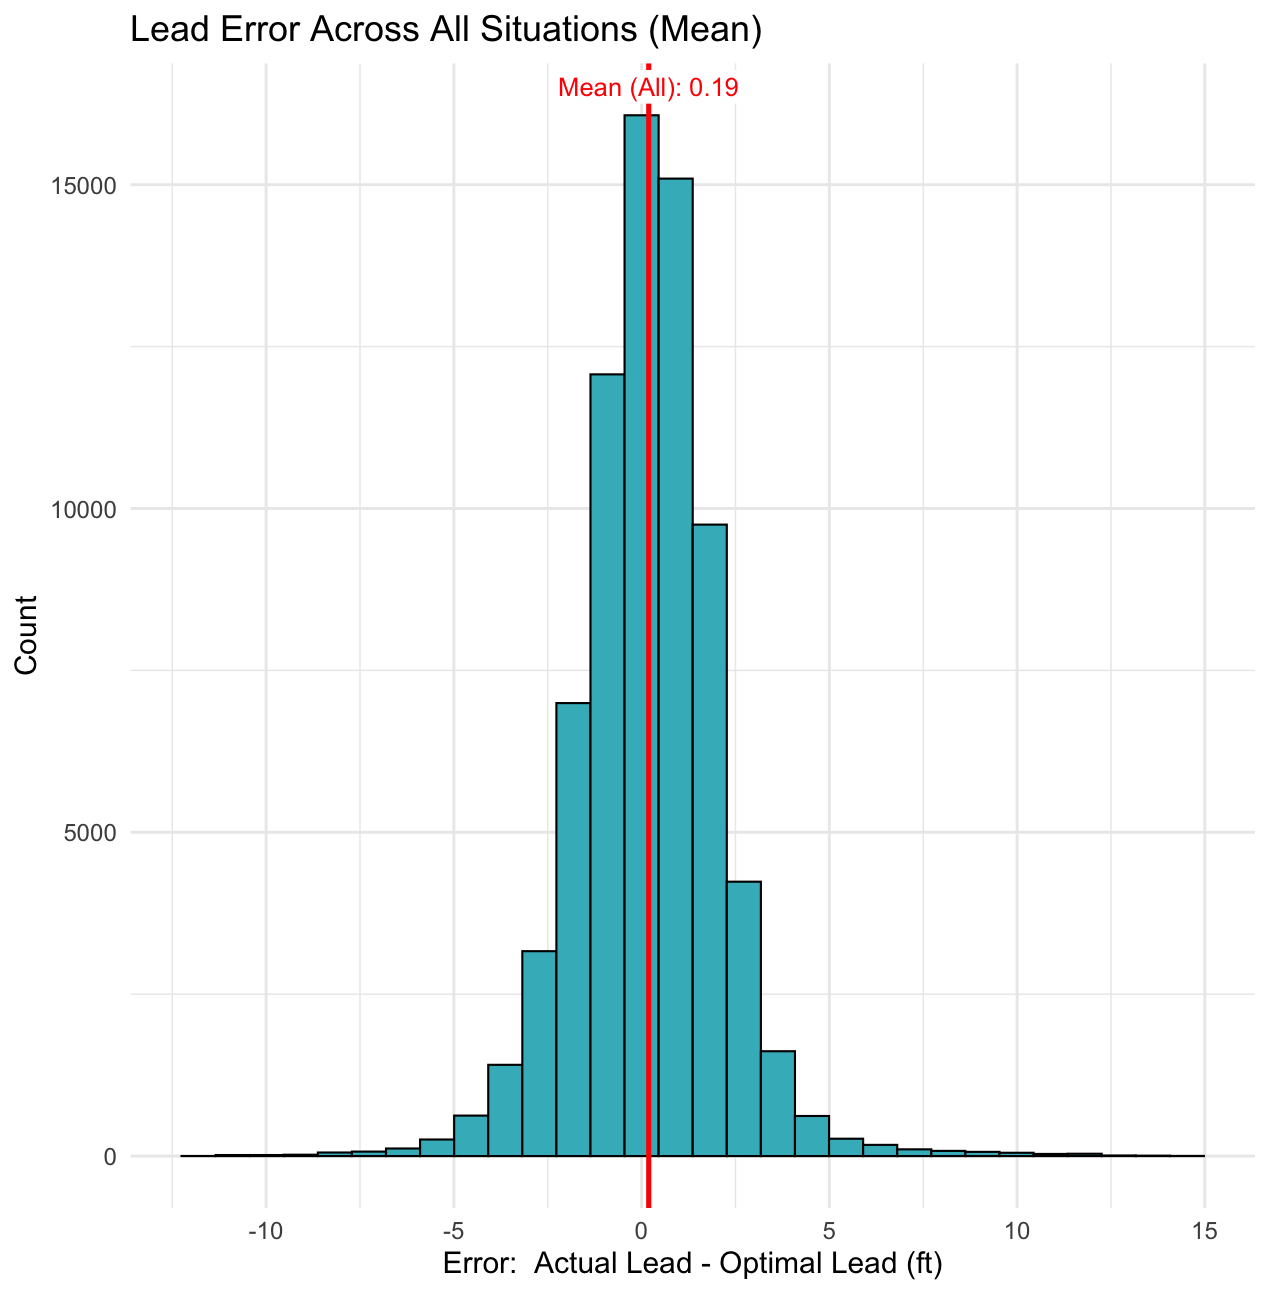
\includegraphics[width=0.8\textwidth]{figures/lead-error-all.png}
    \caption{Distribution of lead deviations across all situations.}
    \label{fig:deviation_all}
\end{figure}

\begin{figure}[!htbp]
    \centering
    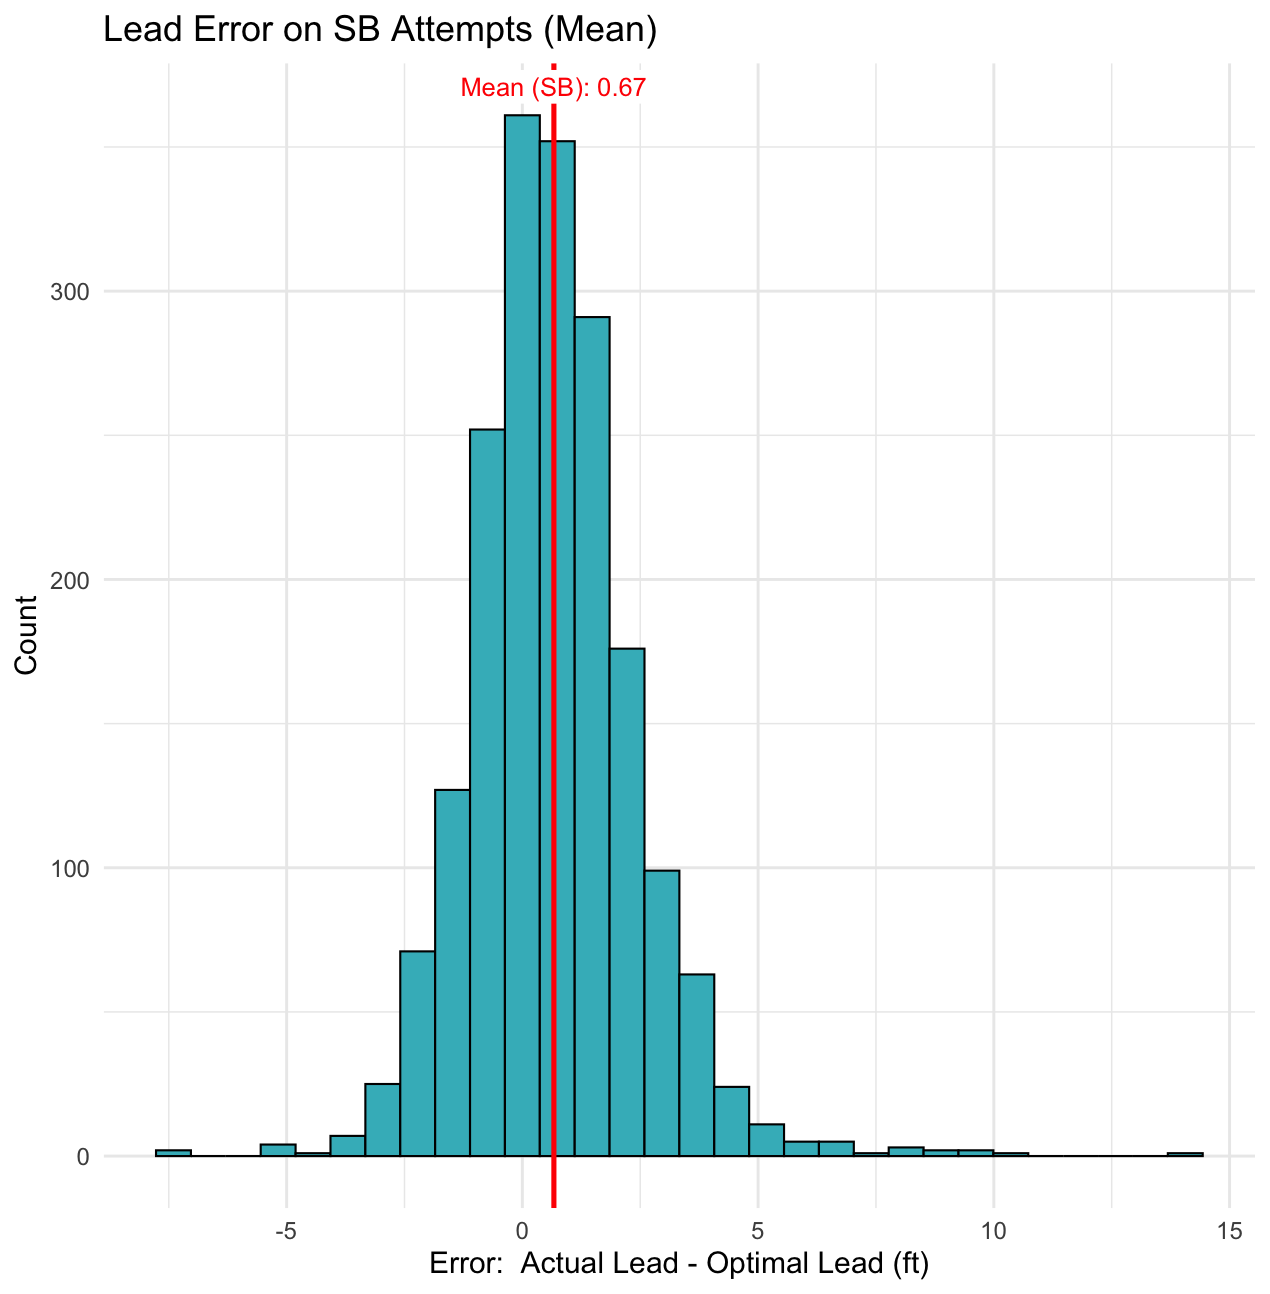
\includegraphics[width=0.8\textwidth]{figures/lead-error-sb.png}
    \caption{Distribution of lead deviations when a stolen base is attempted. Note that this distribution has a higher center than the distribution across all situations.}
    \label{fig:deviation_sba}
\end{figure}

\subsection{Case Study: Cubs vs. Pirates, August 28, 2024}

In an August 28, 2024 game between the Chicago Cubs and Pittsburgh Pirates, Pete Crow-Armstrong (PCA) took an 11.46 foot lead against opposing pitcher Paul Skenes and catcher Yasmani Grandal (pictured in Figure \ref{fig:example_case}). Considering PCA's sprint speed of 30 ft/s, Skenes' estimated Threat of 4.039, and Grandal's pop time of 2.09 seconds, our model produces an optimal lead estimate ($L^*$) of 10.37 ft. PCA's lead exceeds this estimate by 1.09 feet, indicating a slightly more aggressive lead than recommended.

Figure \ref{fig:implied_probs} displays the model-implied probabilities of SB, CS, and PK as functions of primary lead $L$ given the players involved, as well as the expected-runs estimate xRuns($L$). Figure \ref{fig:optimal_lead} demonstrates that a lead distance of 10.37 ft maximizes estimated expected runs (+0.007). This turning point reflects the risk-reward balance when taking a lead: larger leads increase the probability of reaching second safely, at the cost of increased pickoff danger.
 
\begin{figure}[H]
    \centering
    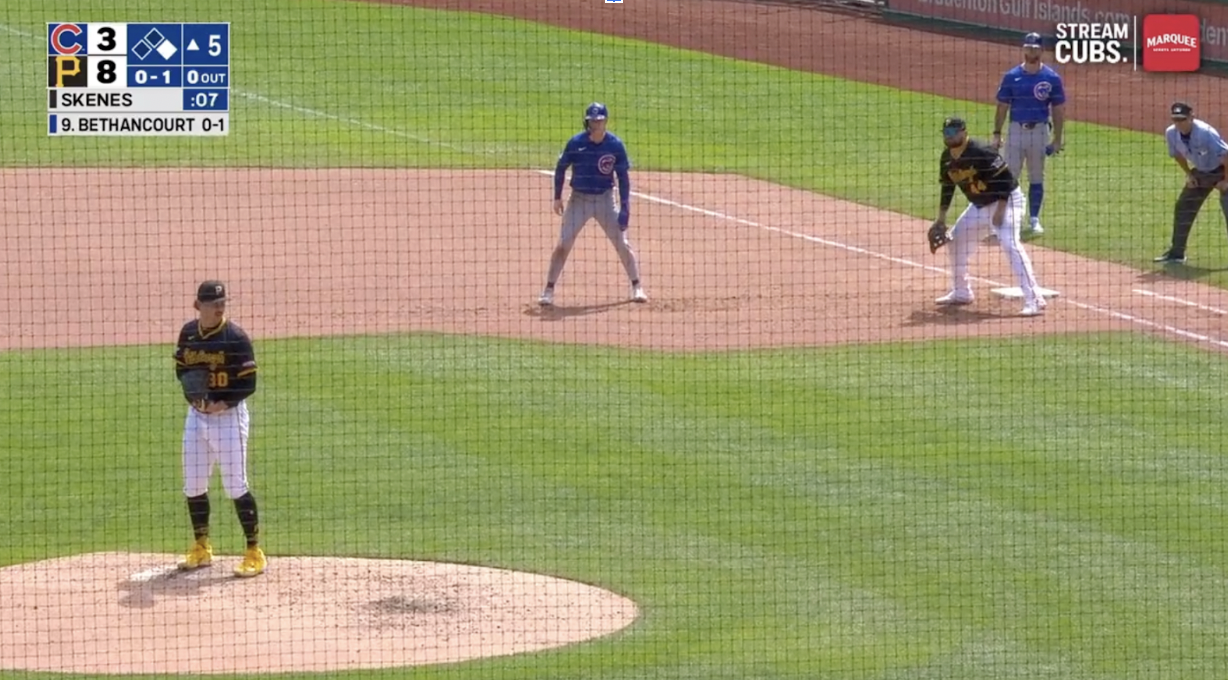
\includegraphics[width=0.9\textwidth]{figures/pca.png}
    \caption{Pete Crow-Armstrong on first base, Paul Skenes pitching, Yasmani Grandal (not seen) catching. \cite{CubsvPirates2024}}
    \label{fig:example_case}
\end{figure}

\begin{figure}[H]
    \centering
    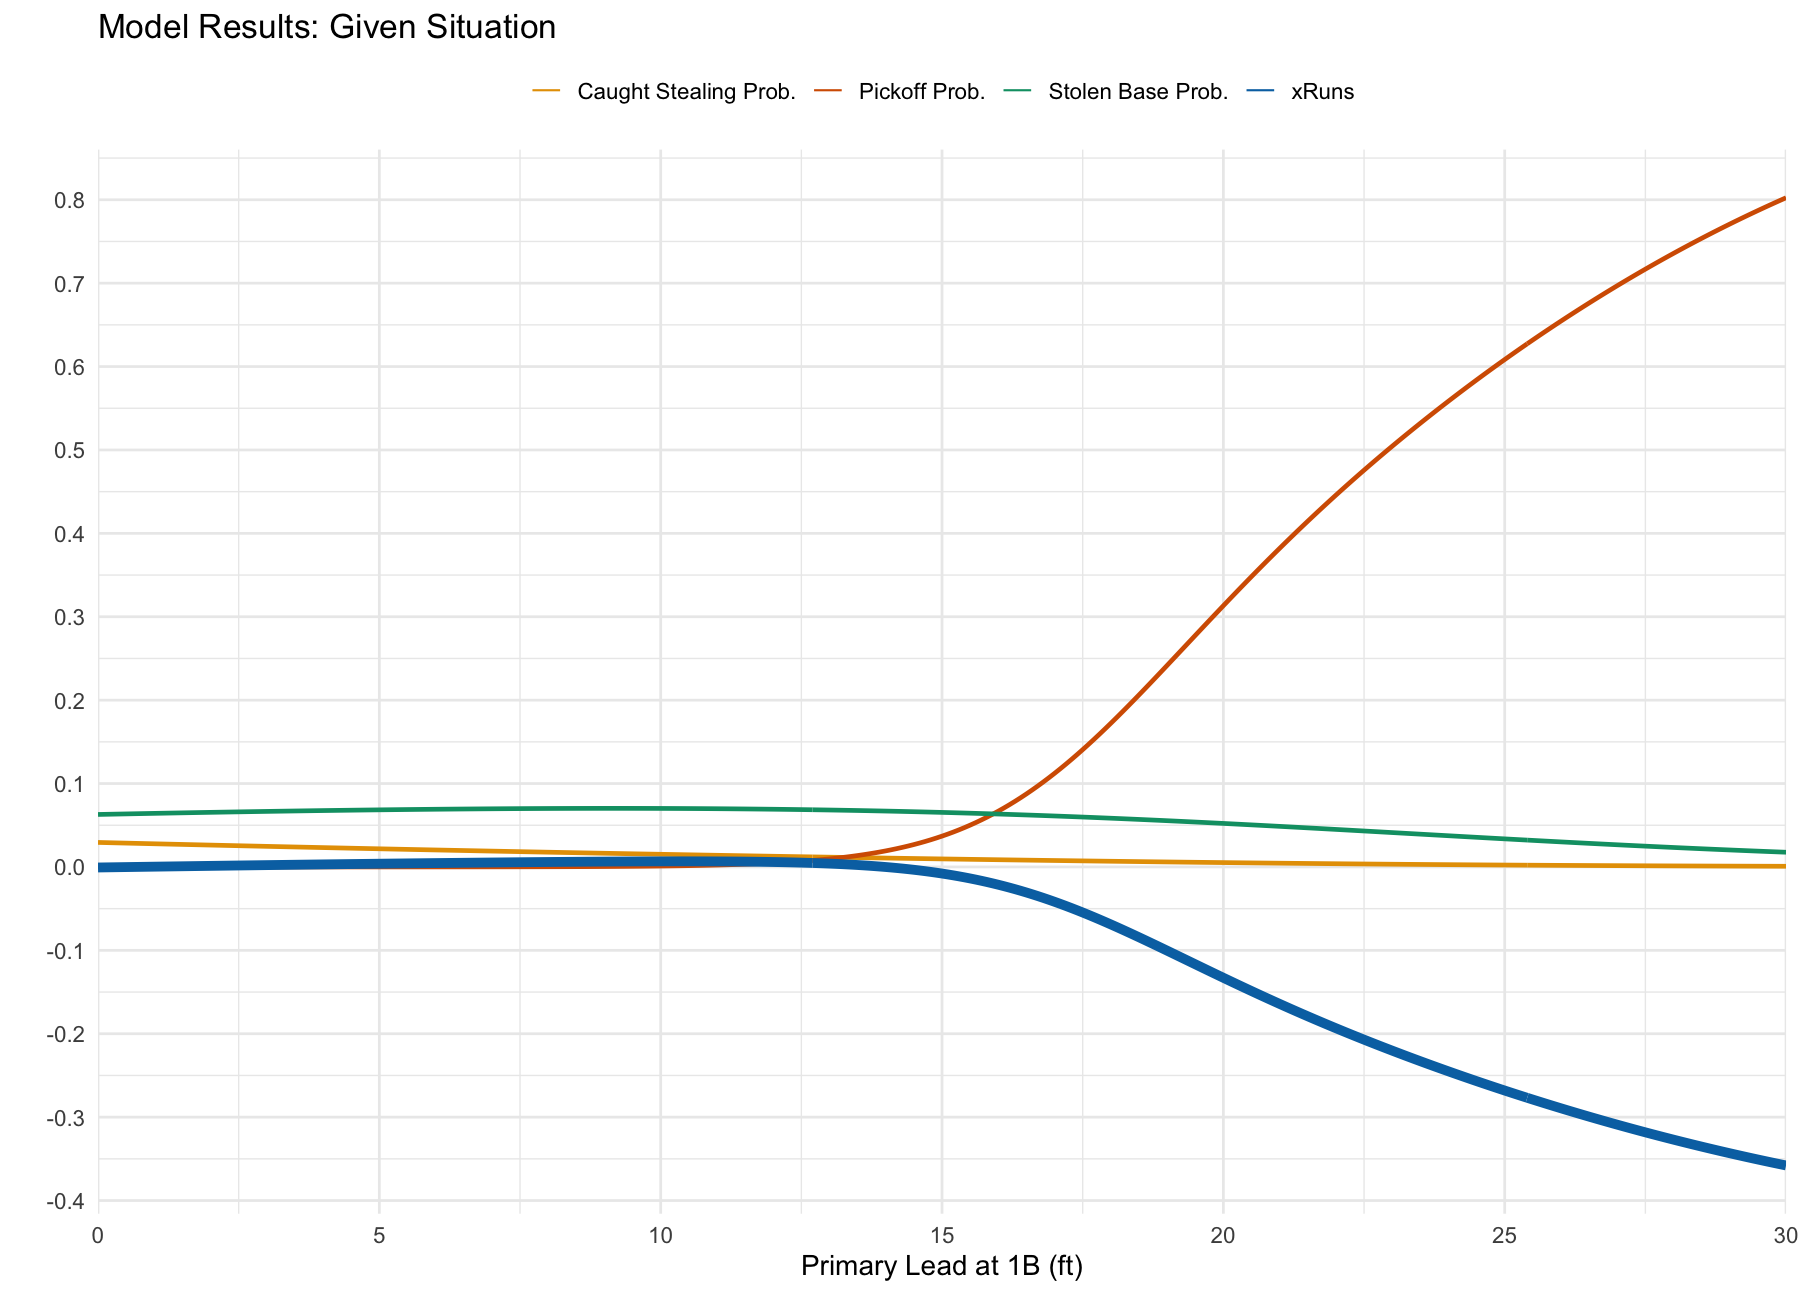
\includegraphics[width=0.8\textwidth]{figures/pca-probs.png}
    \caption{Our model-implied outcome probabilities and estimated xRuns as a function of Pete Crow-Armstrong's lead distance.}
    \label{fig:implied_probs}
\end{figure}
\begin{figure}[H]
    \centering
    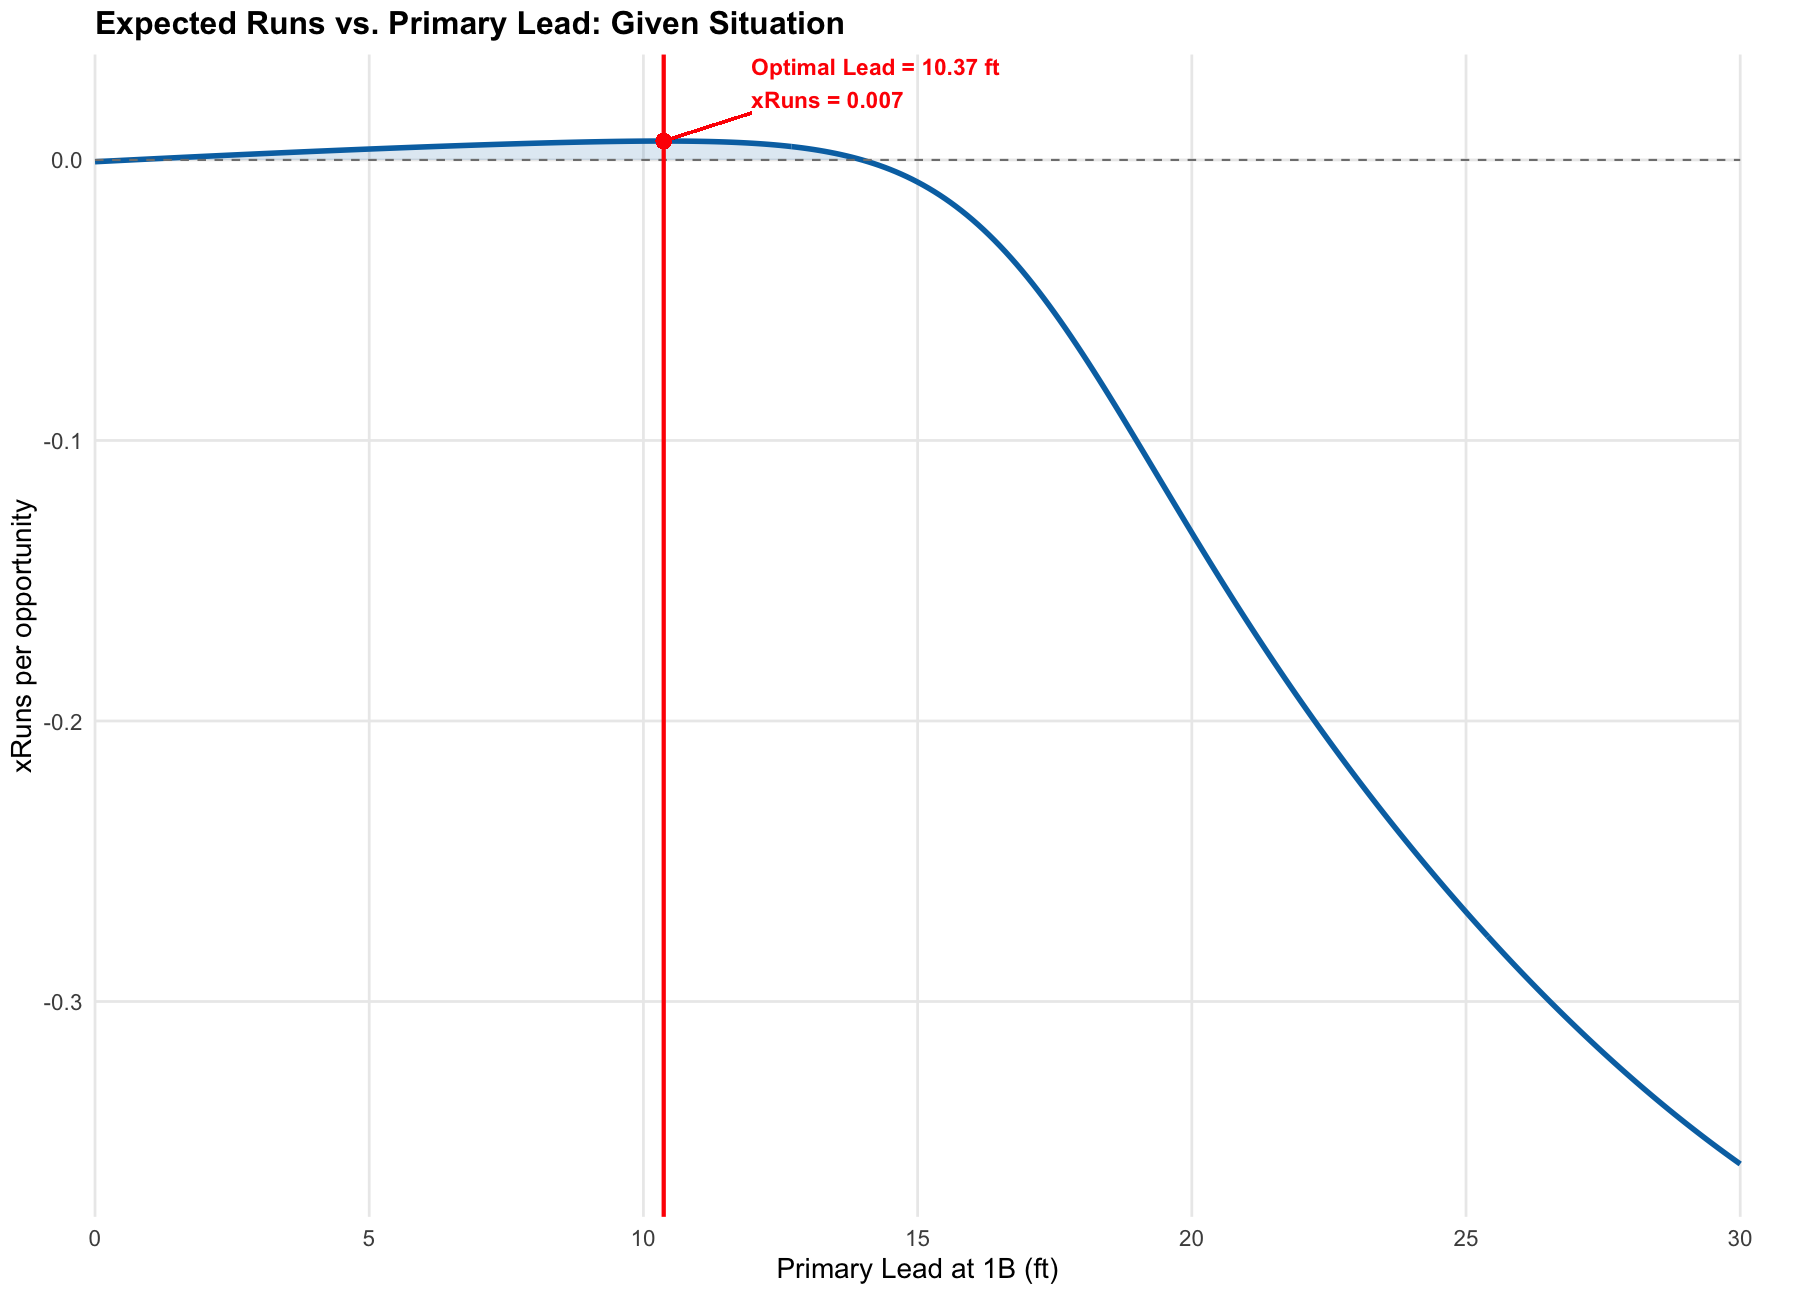
\includegraphics[width=0.8\textwidth]{figures/pca-xruns.png}
    \caption{Expected runs as a function of Pete Crow-Armstrong's lead distance.}
    \label{fig:optimal_lead}
\end{figure}

\section{Discussion}

\subsection{Conclusions}

This study proposes a tractable framework for selecting a primary lead off first base that \emph{maximizes expected runs} in the base state with a runner on first and second/third empty. We model the baserunning sequence with nested logistic regressions, using runner sprint speed, catcher pop time, and pitcher hold ability ("Threat"). By mapping stage probabilities to expected runs and evaluating over the observed range of lead distances, we obtain a context-specific optimal lead $L^*$ and a diagnostic measure of deviation ($L^\text{obs}-L^*$).

Our results capture the central trade-off in lead-taking: increasing lead length raises the probability of a successful steal, but also increases pickoff risk, yielding an xRuns($L$) profile with a well-defined maximum. Empirically, observed leads are modestly larger than optimal on average ($\approx$ +0.19 ft), with a greater departure on steal attempts ($\approx$ +0.67 ft), which we believe is consistent with unobserved intent to steal.

These findings offer an interpretable, data-driven basis for calibrating lead size that connects directly to run expectancy, recovering intuitive effects and yielding stable recommendations within the observed support.

\subsection{Limitations and Future Directions}

Our analysis is not without its limitations, and each suggests a direct extension. Most importantly, we do not observe \emph{intent to steal} on a given pitch, and lead distance $L$ may co-move with intent. In practice, clubs know when a runner has a green light to steal, and with access to intent labels could sharpen estimates by including that as a predictor. We also restrict attention to the base state with a runner on first and second/third empty; other configurations will shift both expected-run payoffs and defensive behavior, which could be addressed by a parallel analysis. Furthermore, we map outcomes to expected runs using \emph{context-averaged linear weights} for ease, though the true value of a steal depends on game state. Substituting in context-dependent expected run calculations from a table like Table \ref{tab:re24} would yield situation-specific recommendations. Our model also treats each pitch as independent, though we know pitchers and runners adapt within at-bats and games. Finally, our data includes only pickoffs and a sample of called pitches, under-representing swing outcomes. A similar analysis with more extensive data (including other plausibly-important covariates like pitcher/batter handedness, pitch type/location, etc.) would correct for this.

\subsection{Reproducibility}

All analysis code and figure scripts are available \href{https://github.com/wharton-moneyball/stolen-base-leads}{HERE}. Proprietary MLB data are not publicly available.

\section{Acknowledgments}

We would like to thank Moneyball Academy, led by Professor Abraham Wyner and the Wharton Sports Analytics and Business Initiative (WSABI), for supporting this research. We are also grateful to Major League Baseball for providing the data. We would also like to thank Jonathan Pipping, Noah Sonnenklar, and Adam Kuechler for their generous mentorship and guidance, and our teammates, Will Diflorio and Jackson Hubbard, for their contributions over the summer.

\bibliographystyle{apalike}
\bibliography{references}

\appendix

\section{Additional Lead Deviation Visualizations} \label{app:a}

Figure~\ref{fig:deviation_by_team} reports the \emph{mean absolute lead deviation} by team across all runner-on-first events. Lower values indicate closer adherence to the model’s optimal lead. In our sample, the Philadelphia Phillies and St.~Louis Cardinals exhibit the largest mean absolute deviations, whereas the Minnesota Twins, Detroit Tigers, and Atlanta Braves cluster near zero (closest to optimal).

Figure~\ref{fig:runners_closest} displays the runners with the smallest \emph{absolute} mean lead deviation (i.e., most consistently near-optimal). Figure~\ref{fig:runners_tails} shows the tails of the signed distribution: panel~(a) lists the most \emph{aggressive} runners (positive mean deviation; leads longer than optimal) and panel~(b) lists the most \emph{conservative} runners (negative mean deviation; leads shorter than optimal). Jazz Chisholm Jr., Michael Conforto, and Dansby Swanson obey our model most closely (on average). Daniel Vogelbach, Mike Ford, and Luken Baker take the most aggressive leads on average, while  Brooks Baldwin, Anthony Volpe, and Carlos Correa take the most conservative leads on average.

\begin{figure}[!htbp]
    \centering
    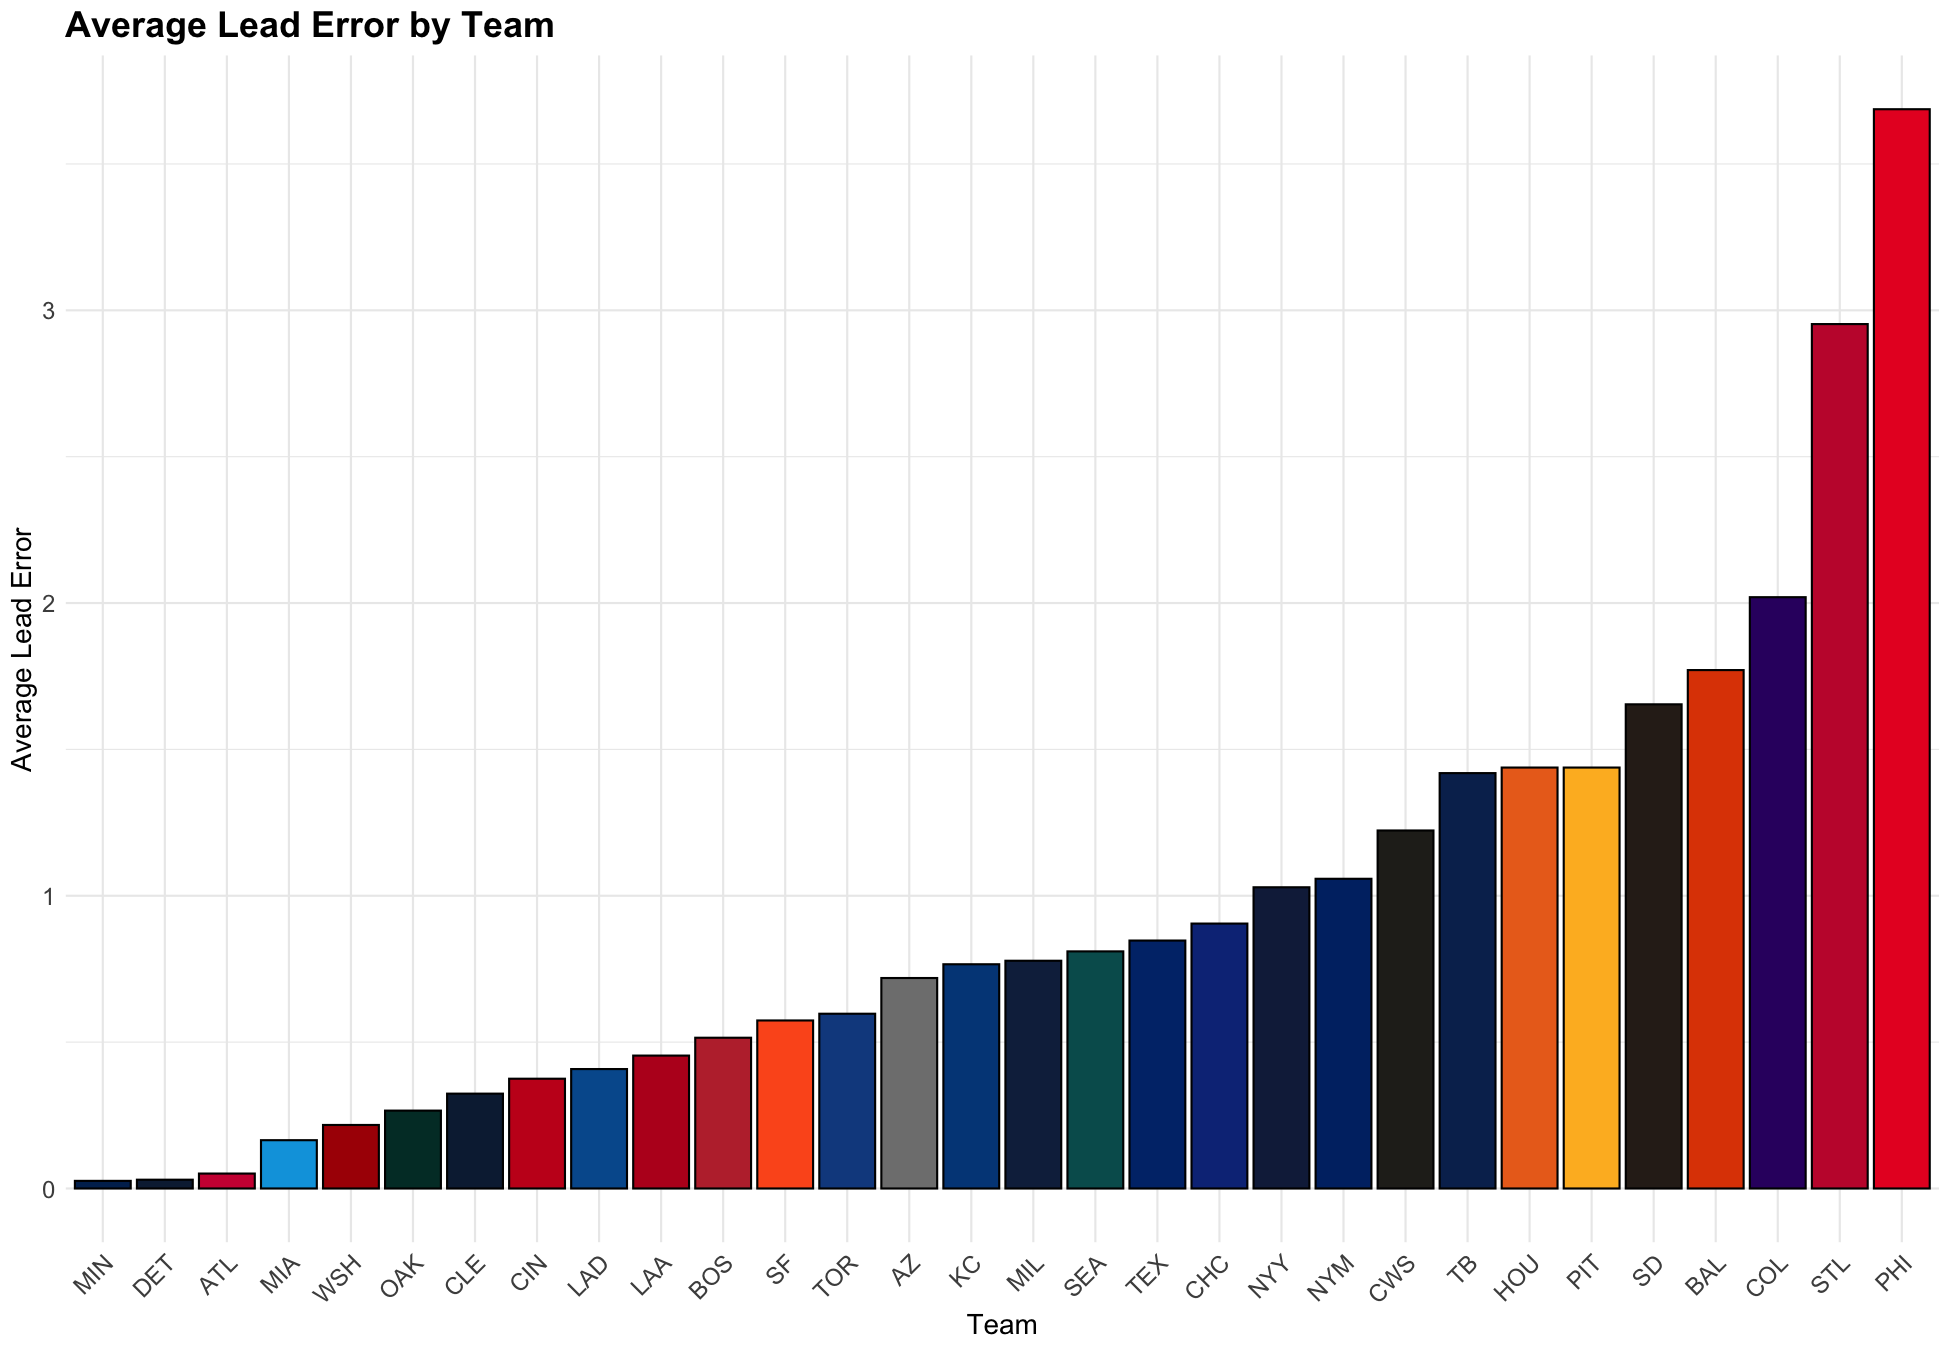
\includegraphics[width=0.9\textwidth]{figures/team-lead-error.png}
    \caption{Bar plot of average absolute lead deviation by team.}
    \label{fig:deviation_by_team}
\end{figure}

\begin{figure}[!htbp]
    \centering
    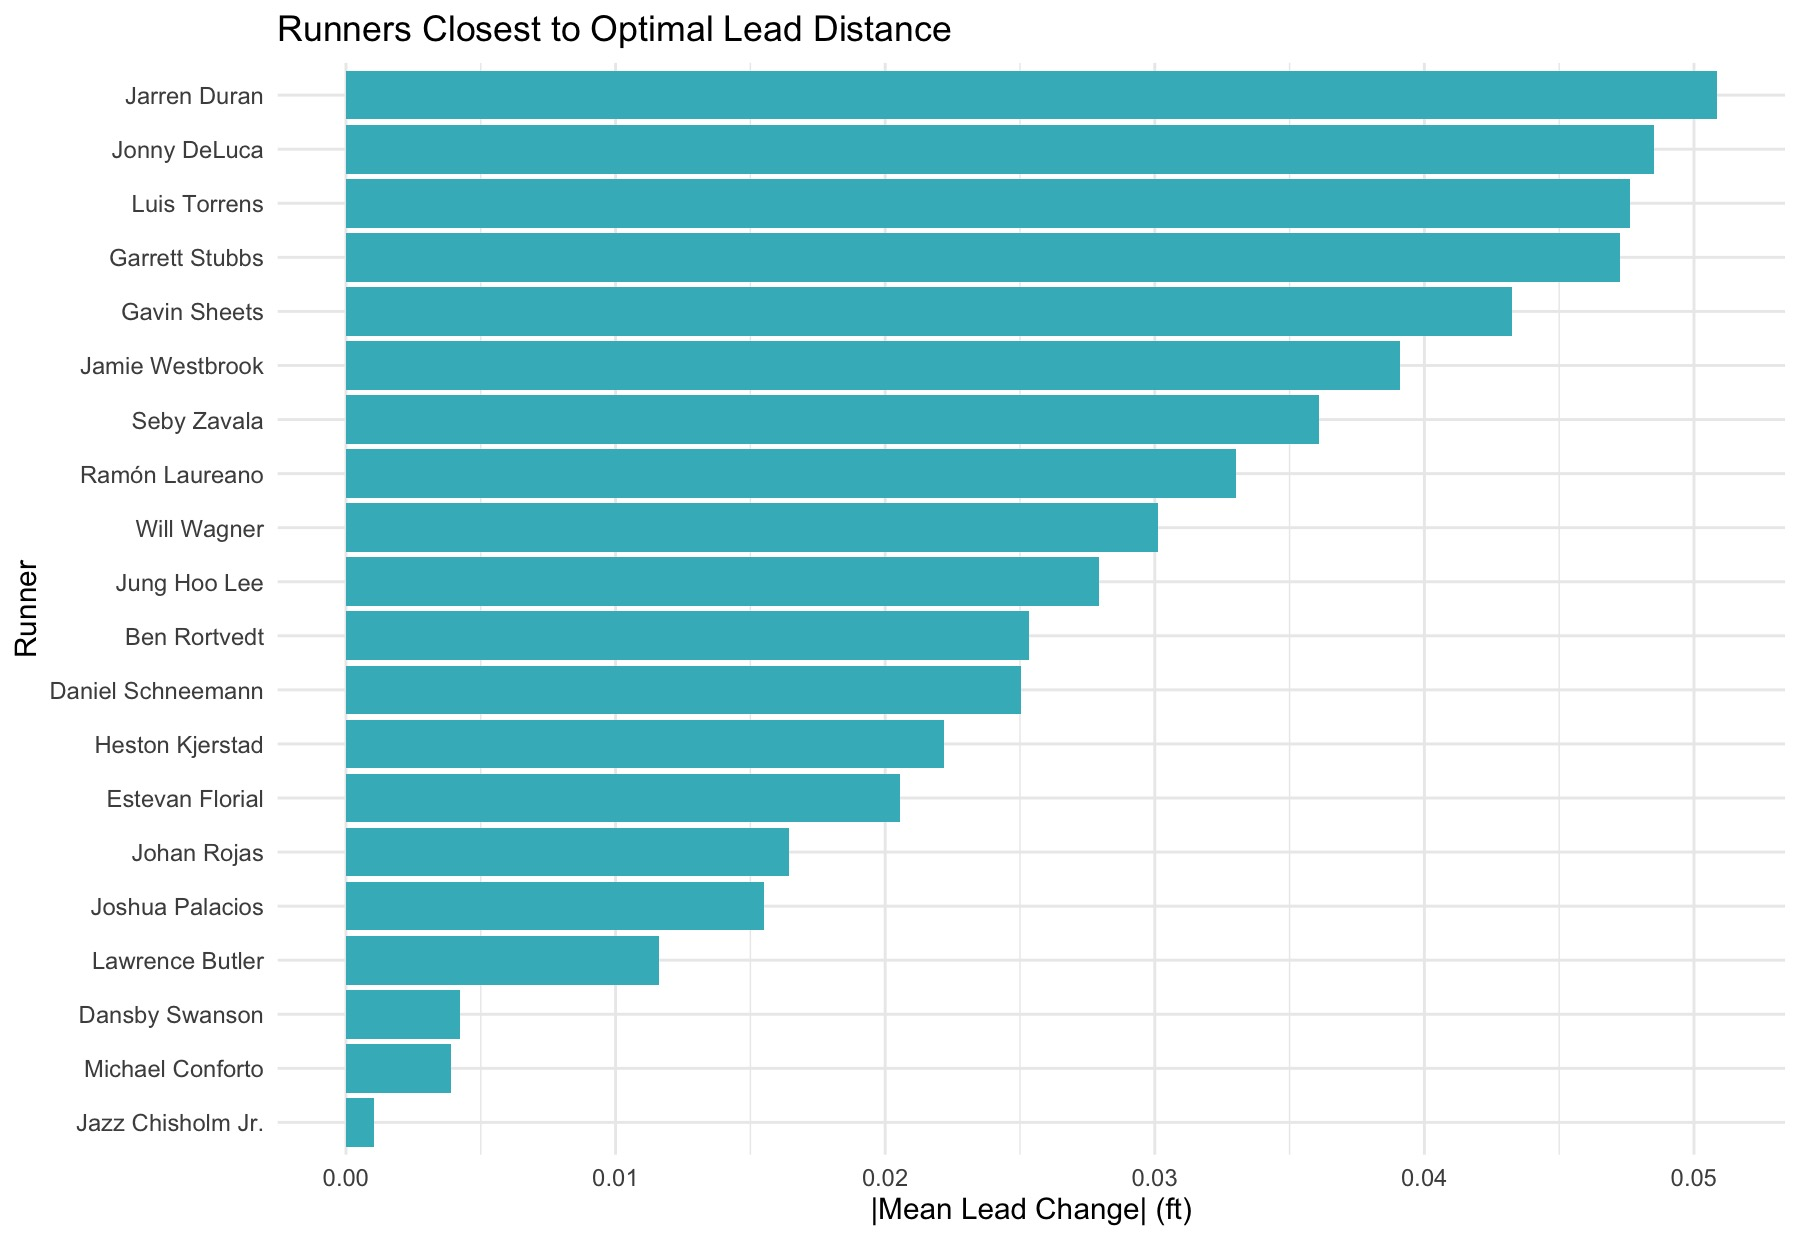
\includegraphics[width=0.8\textwidth]{figures/runners-closest.jpeg}
    \caption{Baserunners with the smallest absolute average lead deviation.}
    \label{fig:runners_closest}
\end{figure}

\begin{figure}[!htbp]
    \centering

    \begin{subfigure}[t]{0.6\textwidth}
        \centering
        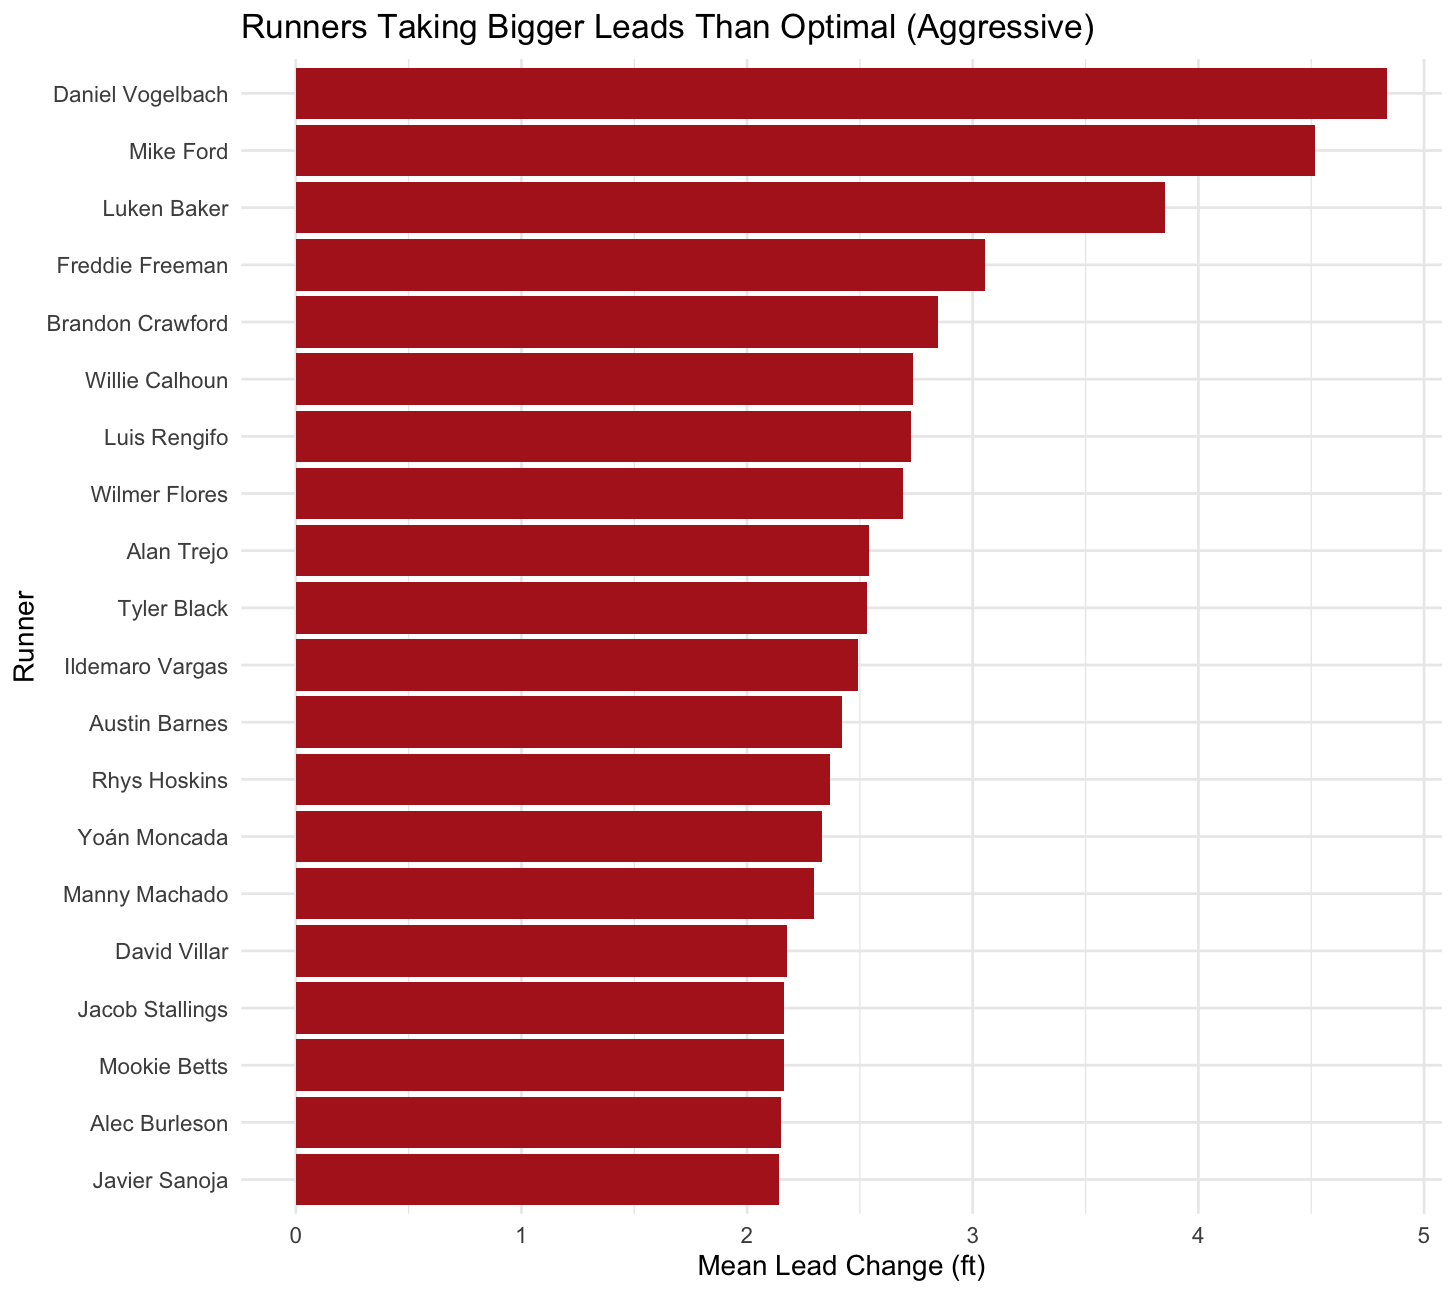
\includegraphics[width=\linewidth]{figures/bigger-leads.png}
        \caption{Baserunners with the most positive average lead deviation.}
        \label{fig:runners_aggressive}
    \end{subfigure}

    \vspace{0.7em}

    \begin{subfigure}[t]{0.6\textwidth}
        \centering
        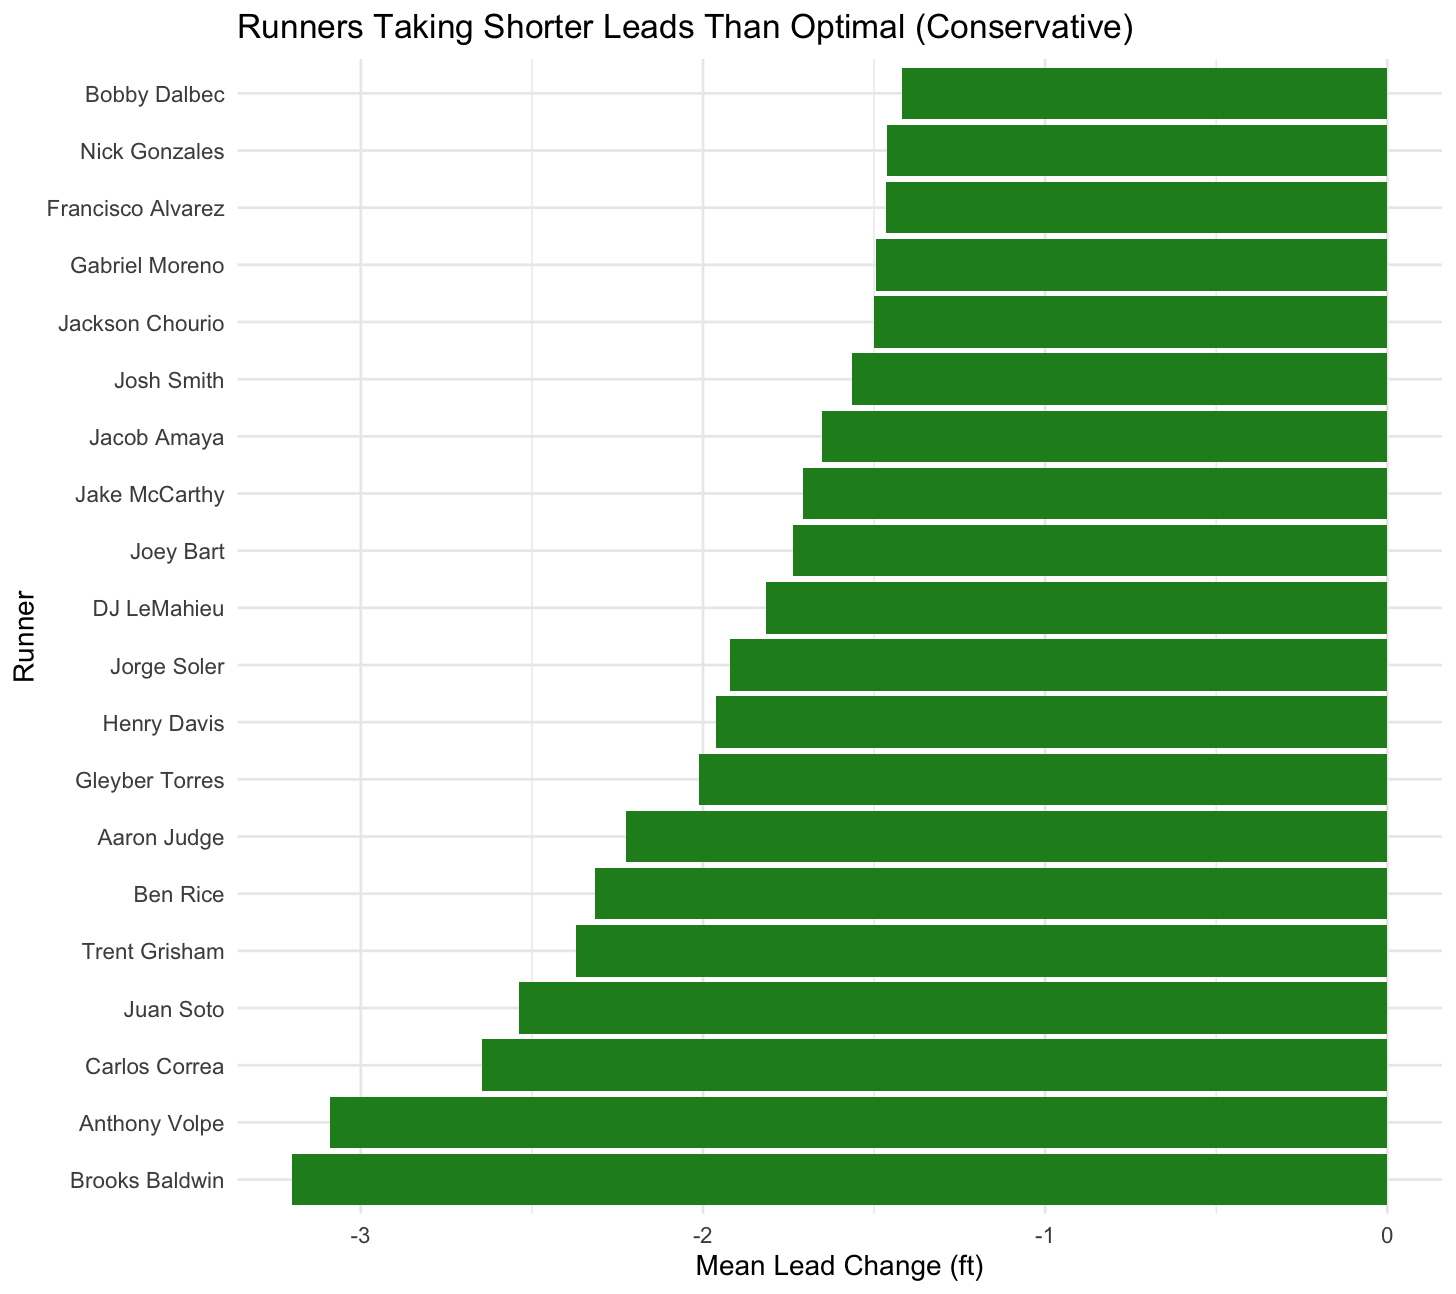
\includegraphics[width=\linewidth]{figures/shorter-leads.png}
        \caption{Baserunners with the most negative average lead deviation.}
        \label{fig:runners_conservative}
    \end{subfigure}

    \caption{Baserunners with the largest signed lead deviations: (a) aggressive (longer-than-optimal) and (b) conservative (shorter-than-optimal).}
    \label{fig:runners_tails}
\end{figure}


\end{document}